\chapter{Considerações Gerais}
\label{cap:02}
\begin{comment}



Texto das considerações gerais, dividido em subseções.

Este é um exemplo de como usar figuras. Referência cruzada: Figura~\ref{fig:exemplo}

\FloatBarrier
\begin{figure}[!htbp]
	\centering
	\caption{Exemplo de figura}
	%scale redimensiona a figura.
	%1.5 = 150% do tamanho original
	%1 = 100% do tamanho original
	%0.20 = 20% do tamanho original
	
\includegraphics[scale=0.4]{imagens/exemploFigura}
	\\\textbf{Fonte:} Elaborada pelo autor
	\label{fig:exemplo}
\end{figure}
\FloatBarrier


Este é um exemplo de como usar tabelas. Referência cruzada: Tabela~\ref{tab:exemplo}

\FloatBarrier
\begin{table}[!htbp]
	\centering
	\caption{Exemplo de tabela de 2 colunas}
	\begin{tabular}{ c | c }
		\hline
		\textbf{Coluna 1} & \textbf{Coluna 2} \\ \hline
		Dado 1a           & Dado 2a           \\ \hline
		Dado 1b           & Dado 2b           \\ \hline
		Dado 1c           & Dado 2c           \\ \hline
		Dado 1d           & Dado 2d           \\ \hline
	\end{tabular}
	\\ \vspace{0.2cm}
	\textbf{Fonte:} Elaborada pelo autor
	\label{tab:exemplo}
\end{table}
\FloatBarrier


Este é um exemplo de como usar quadros. Referência cruzada: Quadro~\ref{qua:exemplo}

\FloatBarrier
\begin{quadro}[!htbp]
	\centering
	\caption{Exemplo de quadro}
	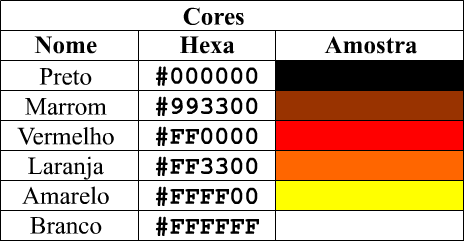
\includegraphics[scale=.7]{imagens/exemploQuadro}
	\\\textbf{Fonte:} Elaborada pelo autor
	\label{qua:exemplo}
\end{quadro}
\FloatBarrier


Este é um exemplo de como usar equações. Referência cruzada: Equação~\ref{eq:exemplo}

\begin{equation}
\sum_{i=1}^{n} i = \frac{n(n+1)}{2}
\label{eq:exemplo}
\end{equation}


Exemplo de inserção de lista de código fonte:

\lstinputlisting[language=Java]{fontes/ClasseExemplo.java} 



Este é um exemplo de como inserir texto sem formatação (ambiente verbatim):

\begin{verbatim}
Texto sem formatação, como espaçamento igual.
\end{verbatim}


Exemplo de lista de itens:

\begin{itemize}
	\item \textbf{Item 1:} texto...;
	\item \textbf{Item 2:} texto...;
	\begin{itemize}
		\item \textbf{Subitem:} texto...;
		\item \textbf{Subitem:} texto...;
		\item \textbf{Subitem:} texto...;
	\end{itemize}
	\item \textbf{Item 3:} texto...;
	\item \textbf{Item n:} texto....
\end{itemize}


Exemplo de lista numerada:

\begin{enumerate}
	\item \textbf{Item:} texto...;
	\item \textbf{Item:} texto...;
	\begin{enumerate}
		\item \textbf{Subitem:} texto...;
		\item \textbf{Subitem:} texto...;
		\item \textbf{Subitem:} texto...;
	\end{enumerate}
	\item \textbf{Item:} texto...;
	\item \textbf{Item:} texto....
\end{enumerate}


Exemplos de comandos para texto e referências:

\begin{itemize}
	\item Para iniciar um novo parágrafo, basta deixar uma linha em branco no código fonte;
	\item Não force o compilador a pular mais de uma linha, pois terá influência negativa na composição do documento;
	\item Sempre deixe o \LaTeX\ realizar a formatação de parágrafos e posicionamento de elementos;
	\item Utilização de aspas simples (abertura \verb|`|, fechamento \verb|'|): `Texto entre aspas simples';
	\item Utilização de aspas duplas (abertura \verb|``|, fechamento \verb|''|): ``Texto entre aspas duplas'';
	\item Negrito (comando \verb|\textbf|): \textbf{texto em negrito};
	\item Itálico (comando \verb|\textit|): \textit{texto em itálico};
	\item Sublinhado (comando \verb|\underline|): \underline{texto sublinhado};
	\item Negrito e itálico (usar comandos juntos): \textbf{\textit{texto em negrito e itálico}};
	\item Alterar cor do texto (comando \verb|\textcolor{cor}{texto}|):
	\begin{itemize}
		\item Exemplo \verb|\textcolor{red}{texto}|: \textcolor{red}{texto vermelho};
		\item Exemplo \verb|\textcolor[RGB]{255, 102, 0}|: \textcolor[RGB]{255, 102, 0}{texto laranja};
		\item Exemplo \verb|\textcolor[HTML]{006AD7}|: \textcolor[HTML]{006AD7}{texto azul};
	\end{itemize}
	\item Ambiente matemático inline (comando \verb|$ expressão $|): $s = x^2-2x +1$;
	\item Referência normal (comando \verb|\cite|):
	\begin{itemize}
		\item \cite{Agaisse1995};
		\item \cite{Abedi2014};
		\item \cite{BtNomenclature2016};
	\end{itemize}
	\item Referência normal com mais de uma obra (comando \verb|\cite|):
	\begin{itemize}
		\item \cite{Abedi2014, Agaisse1995};
        \item \cite{AgapitoTenfen2014, BtNomenclature2016, Nelson2014};
	\end{itemize}
	\item Referência nome e ano (comando \verb|\citeauthorandyear|):
	\begin{itemize}
		\item \citeauthorandyear{Agaisse1995};
		\item \citeauthorandyear{Abedi2014};
		\item \citeauthorandyear{BtNomenclature2016};
	\end{itemize}
\end{itemize}


Exemplo 1 de citação direta:

\begin{citacao}
	Os 20 aminoácidos usualmente encontrados como resíduos em proteínas contém um grupo $\alpha$-carboxil, um grupo $\alpha$-amino e um grupo R distinto substituído no átomo de carbono $\alpha$. O átomo de carbono $\alpha$ de todos os aminoácidos, com exceção da glicina, é assimétrico e, portanto, os aminoácidos podem existir em pelo menos duas formas estereoisoméricas. Somente os estereoisômeros L, com uma configuração relacionada à configuração absoluta da molécula de referência L-gliceraldeído, são encontrados em proteínas \cite[p. 81]{Nelson2014}.
\end{citacao}

Exemplo 2 de citação direta:

\begin{citacao}
	\textit{These various insecticidal proteins are synthesized during the stationary phase and accumulate in the mother cell as a crystal inclusion which can account for up to 25\% of the dry weight of the sporulated cells. The amount of crystal protein produced by a B. thuringiensis culture in laboratory conditions (about 0.5 mg of protein per ml) and the size of the crystals (24) indicate that each cell has to synthesize $10^6$ to $2 \times 10^6$ $\delta$-endotoxin molecules during the stationary phase to form a crystal} \cite[p. 1]{Agaisse1995}.
\end{citacao}

Exemplo de nota de rodapé\footnote{Essa é uma nota de rodapé!}.

\end{comment}

\section{O que é um Jogo?}
Criar e participar de jogos desde os períodos mais
antigos da história é um impulso básico do Homo 
sapiens, desde nossos ancestrais mais remotos,
passando por civilizações como os gregos e os 
romanos, até os dias atuais, sempre existiram 
sistemas e práticas voltados ao ato de jogar, 
tendo como finalidade o entretenimento, a competição
e a educação \cite{egenfeldt2020understanding}.

Um jogo pode ser considerado uma atividade de ocupação
voluntária, realizada dentro de certas limitações de tempo
e espaço, seguindo regras determinadas e obrigatórias, 
com o objetivo de alcançar uma meta específica, gerando
sensações de tensão, desafio e alegria \cite{vasques2025jogar}.

O primeiro jogo eletrônico da história foi lançado em 1958,
chamado Tennis for Two, seu objetivo era simular uma quadra
de tênis 2D e ele foi criado exclusivamente para entretenimento,
permitindo que duas pessoas jogassem presencialmente. Com o
passar dos anos, os jogos foram evoluindo e passaram a ser exibidos
em telas de televisão e computadores, com imagens mais dinâmicas, 
recursos sonoros aprimorados e maior exigência de habilidade e 
aprendizado por parte dos jogadores.

No livro ``Understanding Video Games: The Essential Introduction''
\cite{egenfeldt2020understanding}, os autores explicam que existem
diversas metodologias de análise do que é jogo, sendo três os principais
elementos:

\begin{enumerate}
	\item \textbf{Regras:} O game design que define a estrutura do jogo;
	\item \textbf{Experiência Humana:} O grau de envolvimento e imersão do jogador;
	\item \textbf{Cultura:}  O contexto no qual o jogo está inserido.
\end{enumerate}

Esses três elementos quando juntos em uma aplicação, definem o que é um jogo,
 o game design vai definir as mecânicas e regras em um contexto que se 
 está inserido que vai auxiliar na experiência humana. 

De acordo com Paul Schuytema, no livro ```Design de Games — Uma Abordagem
Prática'' \cite{schuytema2008design}, um jogo eletrônico é uma forma de 
entretenimento composta por atividades, funções e ações realizadas por 
um jogador, limitado por regras dentro de um universo definido, que resultam 
em uma condição final, o universo e as regras têm a função de dar contexto às 
ações do jogador, além de criar desafios e conflitos.
As decisões e ações do jogador fazem parte do processo que compõe o jogo, 
mas o fator mais importante não é apenas chegar ao final, e sim a experiência
e o envolvimento durante o percurso.

Com base nas definições apresentadas, pode-se considerar que um jogo é
algo criado pelo ser humano, composto por um conjunto de regras e
limitações que estabelecem um desafio e um objetivo específico a ser 
alcançado, no caso de um jogo eletrônico, a definição é similar, mas com a adição 
de que o game design precisa ser bem estruturado, com elementos para 
que os jogadores se envolvam para a chegada do objetivo, 
tornando a experiência de jogar satisfatória, não apenas pela 
conquista do objetivo final, mas por todo o processo.

\section{Tipos de Jogos Tradicionais} %será que eu mudo pra TIpos de jogos Tradicionais??

	\subsection{Jogos de Cartas}
	A categoria de jogos de cartas são aquelas no qual há a interação entre os jogadores através de um baralho de cartas,
	são jogos que requerem uma estratégia para serem jogadas, em torno da análise combinatoria das cartas visiveis aos jogadores ("na mesa")
	e das cartas que está nas mãos dos jogadores, em muitos jogos de cartas pode ter a interação e comunicação entre jogadores, 
	permitindo o blefe, por exemplo o poker \cite{lucchese2009conceituaccao}. 

	Na Figura~\ref{fig:baralhoClassico} é mostrada uma imagem de um baralho clássico que está presente em vários jogos de cartas:

	\FloatBarrier
\begin{figure}[!htbp]
	\centering
	\caption{Cartas de um baralho clássico}
	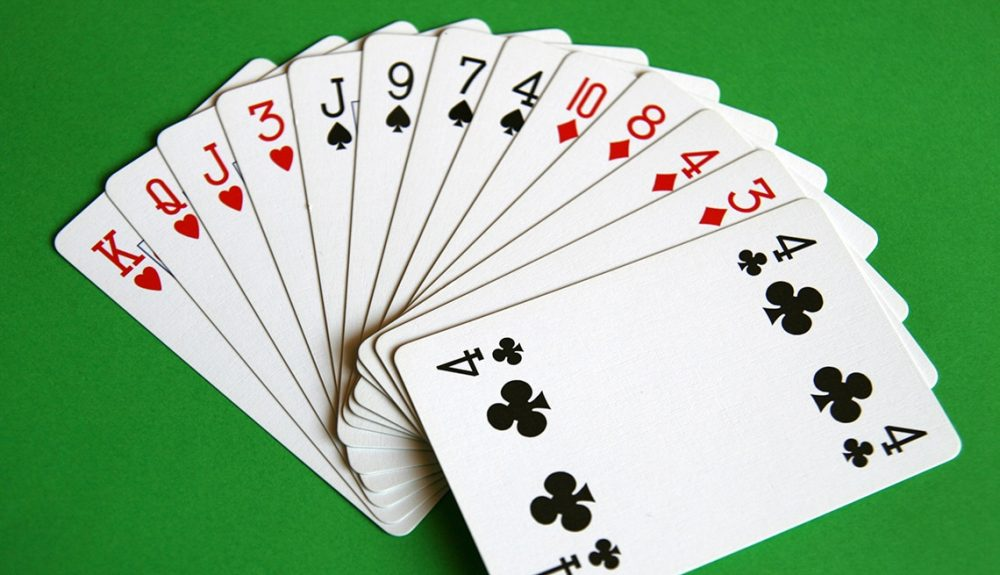
\includegraphics[scale=0.4]{imagens/JogosCartas.jpg}
	\\\textbf{Fonte:} \url{https://segredosdomundo.r7.com/dicas-de-jogos-de-baralho/}
    \label{fig:baralhoClassico}
\end{figure}
\FloatBarrier

	\subsection{Jogos de Tabuleiro}
	Os jogos de tabuleiro são os que representam fisicamente um plano jogavel, divisória de setores
	e um conjunto de peças que podem ser movidas nesse plano ao longo do decorrer do jogo, essas peças devem ser associadas aos jogadores respectivos, em forma ou em cores,
	as estrátegias para ganhar podem variar de jogo para jogo, assim como os objetivos, que podem ser conquistar as peças de outros jogadores, conquistar mais territorios que outros jogadores,
	ter mais pontos ou valores que outros jogadores \cite{lucchese2009conceituaccao}. 
	
	Na figura~\ref{fig:tabuleiroXadrez} é mostrado um exemplo de um jogo de tabuleiro, o xadrez abaixo:

\FloatBarrier
\begin{figure}[!htbp]
	\centering
	\caption{Tabuleiro de Xadrez}
	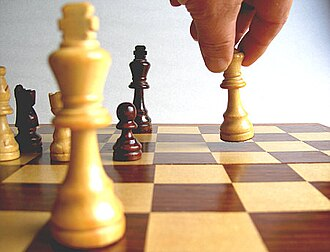
\includegraphics[scale=0.7]{imagens/JogosXadrez.jpg}
	\\\textbf{Fonte:}https://pt.wikipedia.org/wiki/Xadrez
	\label{fig:tabuleiroXadrez}
\end{figure}
\FloatBarrier
	


	\subsection{Jogos de Atléticos}
	Jogos do tipo Atléticos é uma forma tradicional de jogo, eles requerem mais habilidades físicas do que mentais,
	as regras de um jogo atlético requerem que o jogador execute ações precisas, que vai desde jogar uma bola em direção a um adversário,
	 como na Queimada, ou pular de uma altura de 5 metros no salto com vara \cite{gularte2018_oque_e_um_jogo_eletronico}, o uso do corpo e da resistência 
	física é que defini para um jogador ter a habilidade de jogar um jogo atlético. 
	
	Abaixo na figura~\ref{fig:atleticoBasquete} está um exemplo de um jogo atlético, o basquete:
	
\FloatBarrier
\begin{figure}[!htbp]
	\centering
	\caption{Jogo atlético de Basquetebol}
	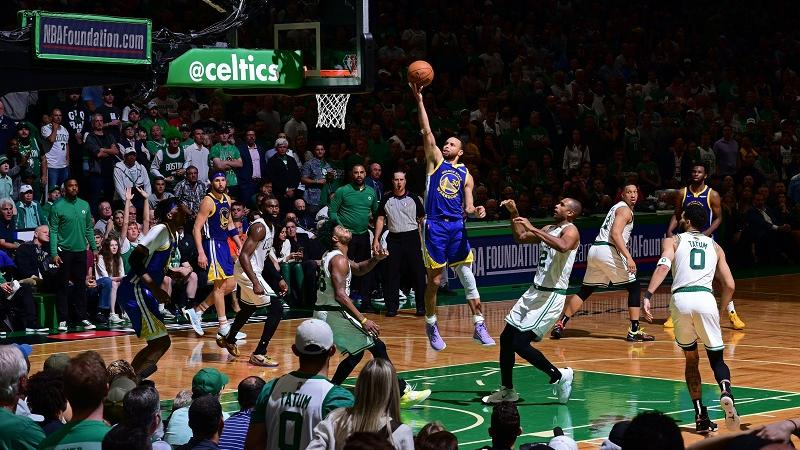
\includegraphics[scale=0.5]{imagens/JogosAtleticos.jpg}
	\\\textbf{Fonte:} https://diariodonordeste.verdesmares.com.br/jogada/com-grande-atuacao-de-curry-golden-state-warriors-bate-celtics-e-conquista-nba-1.3244895
	\label{fig:atleticoBasquete}
\end{figure}
\FloatBarrier

\section{Tipos de Jogos Eletrônicos}

	Nesta seção iremos discorrer a definição dos tipos, genêros e seus subgêneros de jogos eletrônicos, Crawford \cite{crawford1982_art_of_computer_game_design} em seu livro "The Art of Computer Game Design"
	 categorizou os jogos eletrônicos em 2 vertentes, como na figura~\ref{fig:taxodomiaCrawford} abaixo:

	 \FloatBarrier
\begin{figure}[!htbp]
	\centering
	\caption{Classificação de Jogos segundo Crawford}
	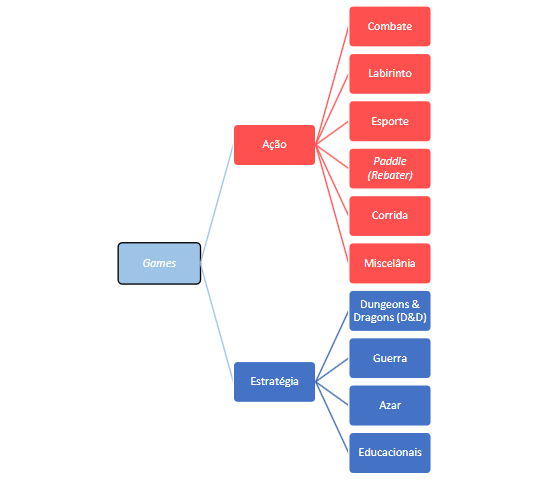
\includegraphics[scale=1.0]{imagens/categoriaGamesCrawford.png}
	\\\textbf{Fonte:} \cite{lucchese2009conceituaccao}
	\label{fig:taxodomiaCrawford}
\end{figure}
\FloatBarrier

	Crawford já havia proposto uma taxonomia dos jogos em 1982, 
	também é possivel observar em materias de divulgação, 
	como no site da CodaKids \cite{codakid2025_video_game_genres} e da Gameopedia \cite{UltimateVideoGames}
	a presença de categorias com caracteristicas semelhantes à de Crawford,
	 o que consolida os genêros e os subgêneros no senso comum dos \textit{videogames}.

	\subsection{Ação}

	Um jogo de ação se catacteriza por requerer do jogador movimentos rápidos,
	com reflexos rápidos, com um ótimo controle visual e tempo de reações rápidos,
	alguns quase instantâneo \cite{UltimateVideoGames, crawford1982_art_of_computer_game_design}.
	\subsubsection{FPS ou \textit{First Person Shooter}}

	Um \textit{First Person Shooter} (Jogo de Tiro em Primeira Pessoa) ou FPS ou Jogos de Tiro se defini através do jogador costantemente
	está mirando e atirando em alvos com a finalidade de alcançar um objetivo.
	Esses jogos se caracterizam por combate entre jogador e inimigo a longas 
	distâncias \cite{UltimateVideoGames}. 
	
	Um clássico dos jogos de FPS é mostrado na figura~\ref{fig:bioshockFPS} abaixo:

\FloatBarrier
\begin{figure}[!htbp]
	\centering
	\caption{Jogo de FPS \textit{Bioshock Infinite}}
	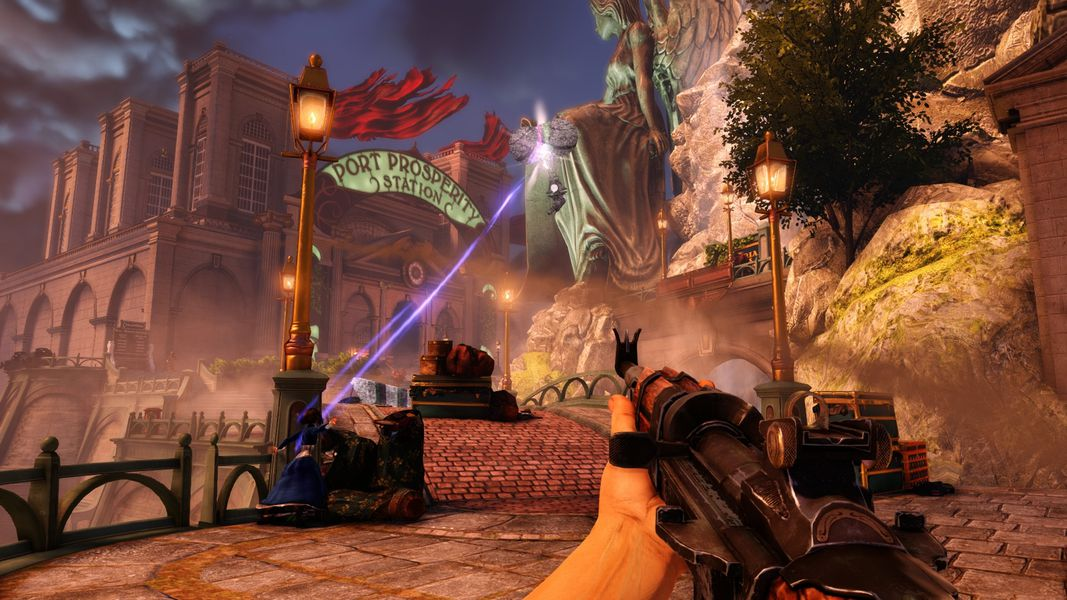
\includegraphics[scale=0.4]{imagens/JogosFPS.jpg}
	\\\textbf{Fonte:} www.imdb.com/es/title/tt1712064/mediaviewer/rm1094737152/
	\label{fig:bioshockFPS}
\end{figure}
\FloatBarrier

\subsubsection{Luta}
Em jogos de luta se caracteriza por um jogador está lutando contra uma máquina ou contra um ou mais jogadores,
é muito comum em jogos de luta, utilizar as teclas que fazem o jogador bater, bloquear, pular encadear sequências de ataques em "combos". 
O combate corpo a corpo está sempre ligado à alguma arte marcial, que está ligado aos personagens do jogo de luta, os jogadores normalmente são representado de lado em um plano 2D, 
há alguns jogos que utilizam planos paralelos no plano 2D para movimentos do jogador \cite{codakid2025_video_game_genres, UltimateVideoGames}. 

Um bom exemplo de um jogo de luta chamado "\textit{Street Figher}"é mostrado na figura~\ref{fig:lutaStreetFighter} abaixo:

\FloatBarrier
\begin{figure}[!htbp]
	\centering
	\caption{Jogo de luta \textit{Street Figher}}
	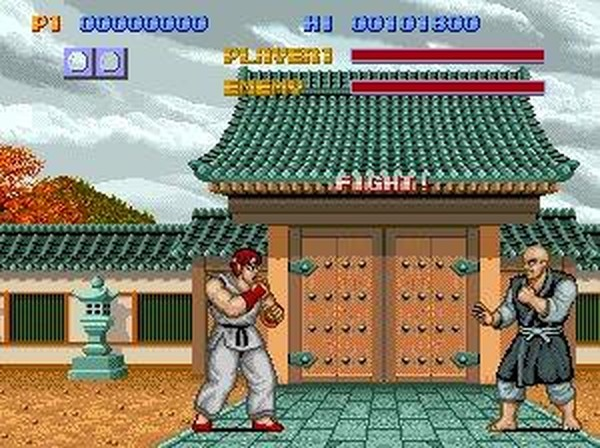
\includegraphics[scale=0.4]{imagens/JogosLuta.jpg}
	\\\textbf{Fonte:}www.techtudo.com.br/noticias/2012/03/especial-a-historia-da-serie-street-fighter-parte-1.ghtml
	\label{fig:lutaStreetFighter}
\end{figure}
\FloatBarrier

\subsubsection{Plataforma}

No subgêneros de jogos de plataforma, os jogadores tem que pular, 
escalar ou usar alguma outra mecânica para se mover de uma plataforma 
até a outra. O jogador deve aprender a lidar inimigos ou evita-los\cite{UltimateVideoGames,codakid2025_video_game_genres}.

É um subgenêro muito consolidado, na década de 1980 com o lançamento de \textit{Super Mario Bros.} e \textit{Donkey Kong}, 
se tornou um subgenêro muito famoso \cite{UltimateVideoGames,codakid2025_video_game_genres}. Um exemplo de jogo de plataforma é mostrado na figura~\ref{fig:plataformaMario} abaixo:

\begin{figure}[!htbp]
	\centering
	\caption{Jogo de Plataforma popular \textit{Super Mario World}}
	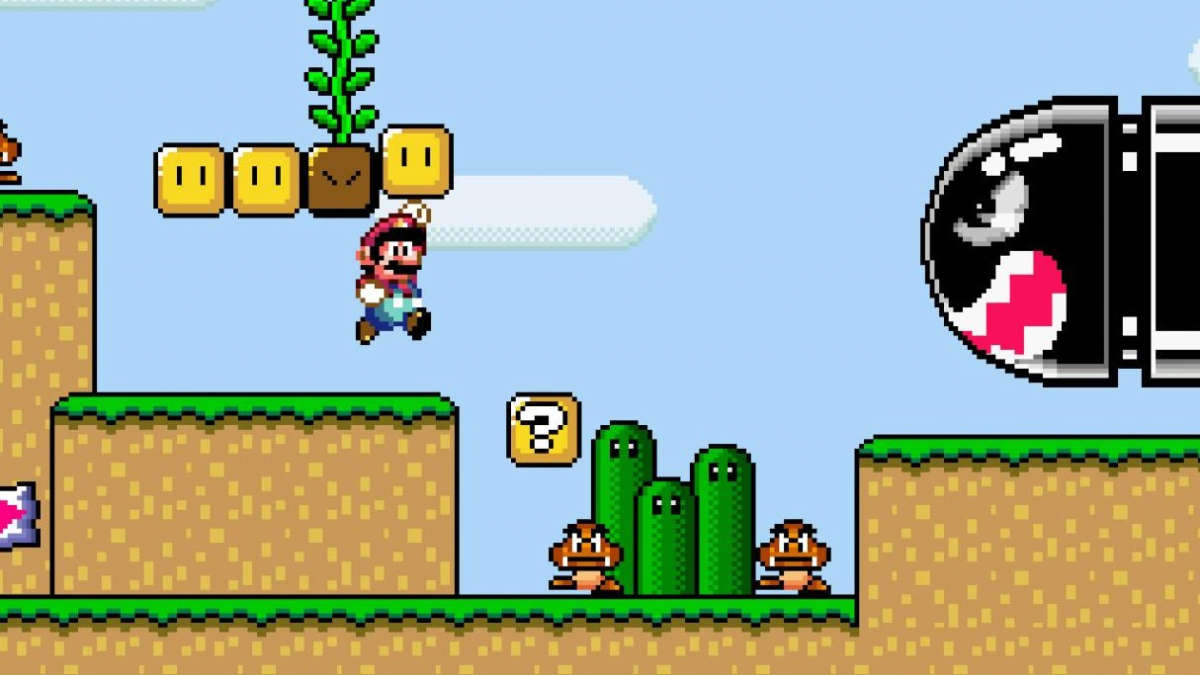
\includegraphics[scale=0.3]{imagens/JogosPlataformas.jpg}
	\\\textbf{Fonte:} https://xboxplay.games/uploadStream/679.jpg
	\label{fig:plataformaMario}
\end{figure}
\FloatBarrier

\subsection{Aventura}

Jogos de aventura se caracterizam-se por oferecer ao jogador a possibilidade de se mover em um cenário ou mundo 
complexo, acompanhado de um enredo estruturado. Ao longo da aventura, o jogador adquire ferramentas e/ou itens e utiliza em 
obstaculos encontrados pelo caminho, resolve quebra cabeças, explora o cenário,
 até atingir um objetivo final ou até chegar ao desfecho da narrativa\cite{crawford1982_art_of_computer_game_design, codakid2025_video_game_genres}, 
uma aventura combina elementos de exploração e narrativa de enredo para serem imersivos ao jogador. \cite{UltimateVideoGames}

Um bom exemplo de jogos de aventura é a franquia de jogos "\textit{The legend of Zelda}", abaixo é mostrado na figura~\ref{fig:aventuraZelda} a imagem de um dos jogos dessa franquia:

\FloatBarrier
\begin{figure}[!htbp]
	\centering
	\caption{Jogo de Aventura \textit{The Legend of Zelda: Ocarina Of Time}}
	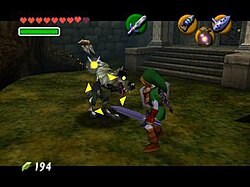
\includegraphics[scale=1.2]{imagens/JogosAventura.JPG}
	\\\textbf{Fonte:} en.wikipedia.org/wiki/ThelegendofZelda
	\label{fig:aventuraZelda}
\end{figure}
\FloatBarrier

\subsection{Ação-Aventura}
Jogos de Ação-Aventura se definem pela combinação de elementos de ação e de aventura, são bem similares a ambos os gêneros,
geralmente oferecem ao jogador uma narrativa construida ao longo de elementos de ação,
o avanço do enredo altamente depende do movimento do personagem do jogador, que desencadeia os eventos da história e afeta o fluxo do jogo \cite{codakid2025_video_game_genres}.
  
Um exemplo de jogo de gênero de ação-aventura é mostrado na figura~\ref{fig:tombraider} abaixo:

  \FloatBarrier
\begin{figure}[!htbp]
	\centering
	\caption{Jogo de ação-aventura \textit{Tomb Raider}}
	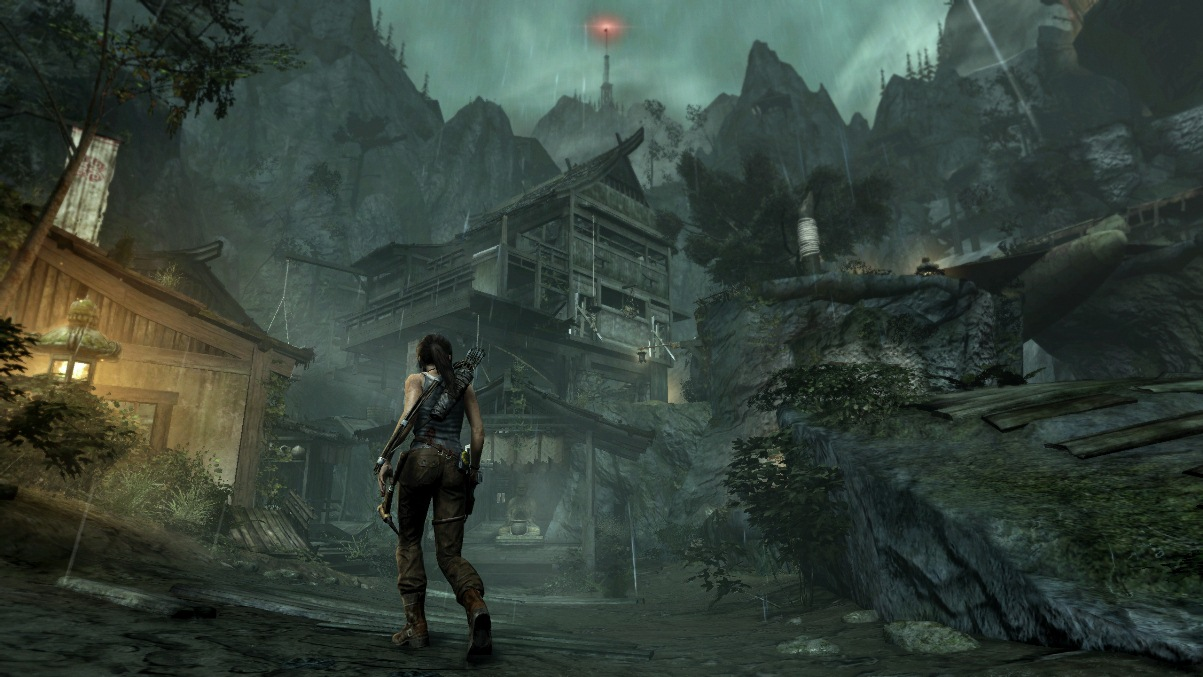
\includegraphics[scale=0.2]{imagens/JogosAcaoAventura.jpeg}
	\\\textbf{Fonte:} https://criticalhits.com.br/reviews/tomb-raider-review/
	\label{fig:tombraider}
\end{figure}
\FloatBarrier

\subsection{\textit{Role Playing Game} ou RPG}
Em um RPG ou Jogo de interpretação de Papeis, o jogador assume um papel de um personagem, criando a aparência 
e evoluindo-o em experiencia e força durante o fluxo do jogo \cite{codakid2025_video_game_genres},
um RPG possibilita o jogador jogar no papel escolhido por ele, por exemplo: em um RPG de fantasia, 
o jogador pode jogar de mago ou de arqueiro, junto de uma narrativa, os jogadores fazem progresso, 
desbloqueiam habilidades, fazer progresso em um RPG, geralmente está amarrado a completar missões que 
está relacionado ao enredo principal e a completar missões secundárias, que não está relacionado ao enredo principal \cite{UltimateVideoGames}.

Um exemplo de um jogo de RPG é mostrado na figura~\ref{fig:rpgTES} abaixo:

\FloatBarrier
\begin{figure}[!htbp]
	\centering
	\caption{Jogo de RPG \textit{The Elders Scrolls: Morrowind}}
	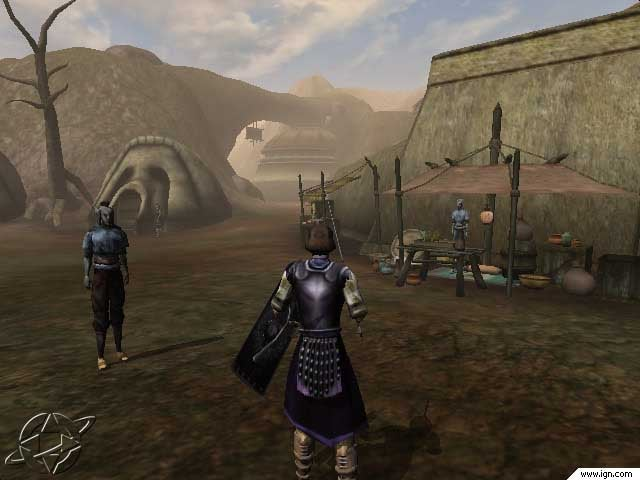
\includegraphics[scale=0.4]{imagens/JogosRPG.jpg}
	\\\textbf{Fonte:} https://www.ign.com/articles/2002/06/17/elder-scrolls-iii-morrowind-review
	\label{fig:rpgTES}
\end{figure}
\FloatBarrier

\subsection{Simulação}

Um jogo de simulação tende a simular ou imitar 
eventos da vida real na forma mais realista possivel \cite{UltimateVideoGames},
a simulação nesses jogos deve assumir diferentes finalidades como educar o jogador, 
permitir análises e previsões, ou simplesmente oferecer entretenimento.
em geral não há um objetivo final delimitado para chegar 
em uma simulação, mas proporciona ao jogador a liberdade para controlar 
um personagem ou o ambiente \cite{codakid2025_video_game_genres}.

Em um jogo de simulação, o jogador precisa estar 
familiarizado com elementos próprios da simulação, 
por exemplo, em \textit{SimCity}, é necessário compreender conceitos relacionados à 
gestão urbana, como as funções de um prefeito e os processos de construção e organização de uma cidade, é mostrado na figura~\ref{fig:simulacaosimcity} uma imagem do jogo abaixo:

%Colocar um jogo de Simulação tipo Sim City ou The sims
\FloatBarrier
\begin{figure}[!htbp]
	\centering
	\caption{Jogo de simulação \textit{Sim City 4}}
	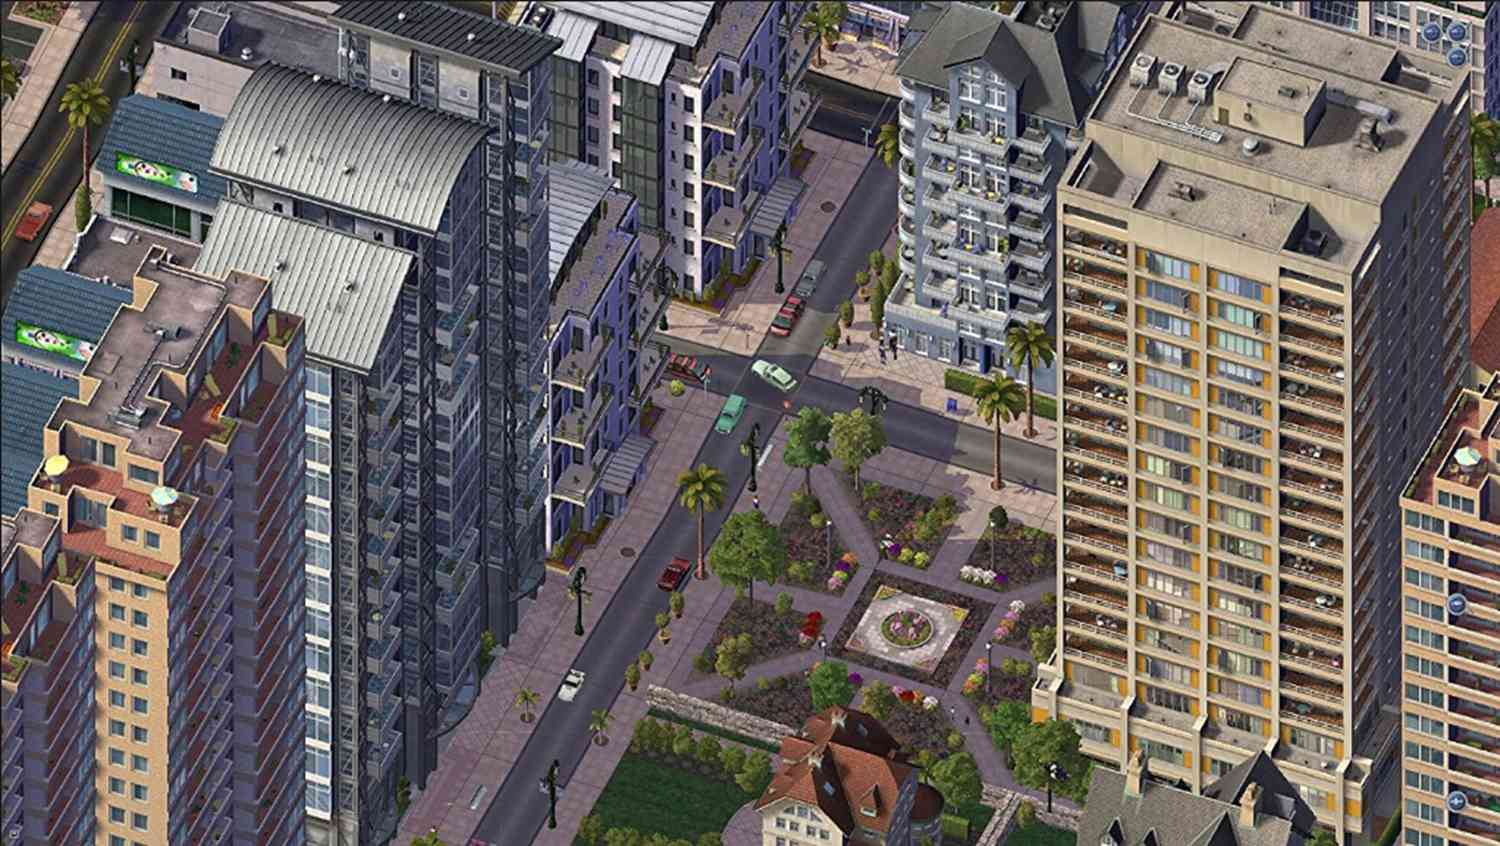
\includegraphics[scale=0.2]{imagens/JogoSimulacao.jpg}
	\\\textbf{Fonte:} https://www.lifewire.com/simcity-4-starting-new-city-840147
	\label{fig:simulacaosimcity}
\end{figure}
\FloatBarrier

\subsection{Estratégia}

Um jogo de estratégia requerem que o jogador pense em planejamento táticos e lógicos tendo como finalidade o objetivo de ganhar \cite{UltimateVideoGames},
o jogador deve realizar uma série de jogadas em turnos contra um ou mais oponentes. Por exemplo, em \textit{StarCraft} o 
jogador deve reunir e distribuir recursos, posicionar tropas nas áreas certas e fornecer a elas os recursos necessários 
para vencer com eficiência, exigindo pensamento táticos e lógica de estratégia\cite{codakid2025_video_game_genres,UltimateVideoGames}.

Um exemplo de um jogo de estratégia é representado na figura~\ref{fig:estrategiainto} abaixo:

\FloatBarrier
\begin{figure}[!htbp]
	\centering
	\caption{Jogo de estratégia \textit{Into The Breach}}
	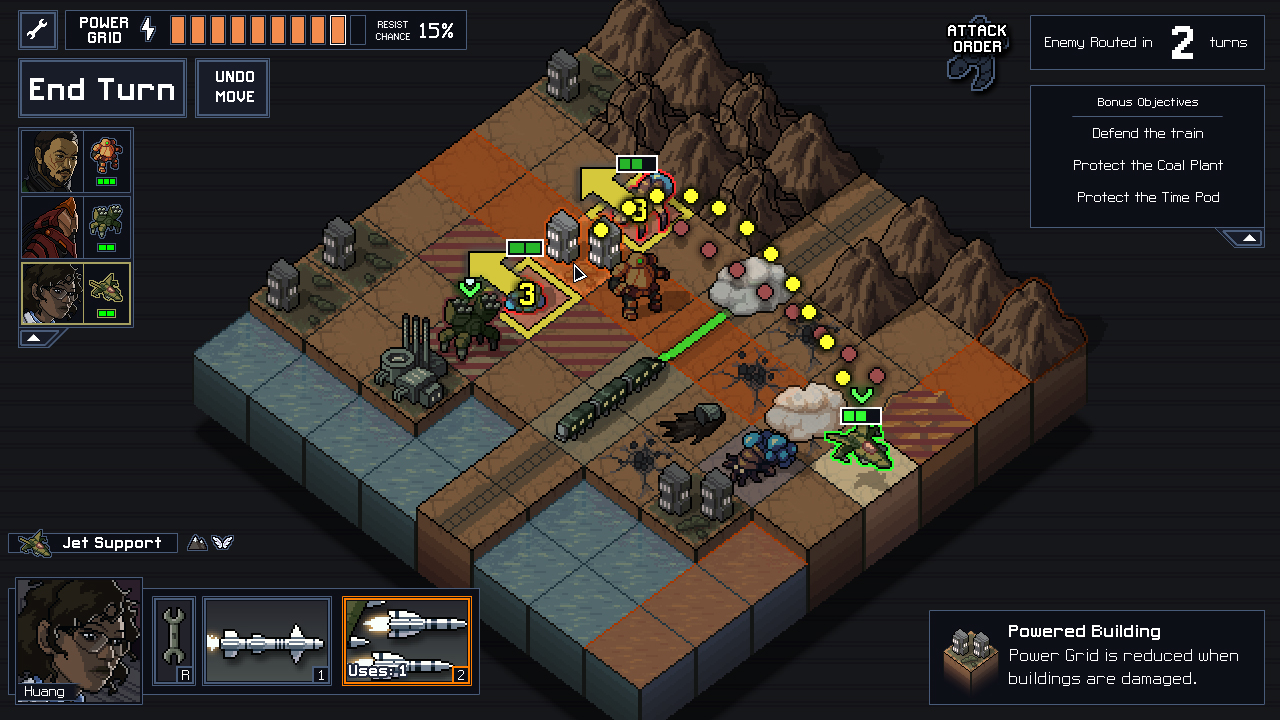
\includegraphics[scale=0.2]{imagens/JogoEstrategia.jpg}
	\\\textbf{Fonte:} https://www.pcgamer.com/into-the-breach-review/
	\label{fig:estrategiainto}
\end{figure}
\FloatBarrier

\subsection{\textit{Puzzle} ou Quebra-Cabeça}

Jogos do tipo \textit{Puzzle} ou quebra-cabeças tem como aspecto central: o jogador resolve problemas utilizando a lógica,
pode haver mais de uma solução em um quebra-cabeça ou em um enigma e um jogador não deve achar a solução aleatóriamente, 
para resolver, o jogador deve reconhecer padrões, descobrir pistas ou até realizar certos movimentos em certas ordens para resolver o quebra-cabeça ou o enigma \cite{UltimateVideoGames}.
Jogos de quebra-cabeça como \textit{Portal} (2007), exigem que o jogador utilize mecânicas de física e manipular portais para passar obstáculos \cite{UltimateVideoGames} e no jogo \textit{Tetris}, exige do jogador organizar peças geométricas em tempo real, testando a agilidade mental e a coordenação espacial, é mostrado um exemplo na figura~\ref{fig:puzzletetris} abaixo:

\FloatBarrier
\begin{figure}[!htbp]
	\centering
	\caption{Jogo de quebra-cabeça \textit{Tetris}}
	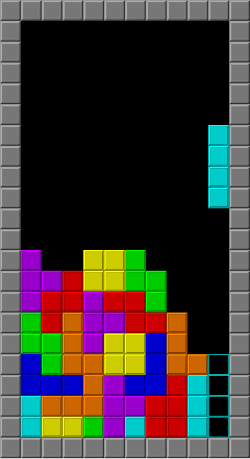
\includegraphics[scale=0.4]{imagens/JogoPuzzle.png}
	\\\textbf{Fonte:} wikipedia.org/wiki/Tetris
	\label{fig:puzzletetris}
\end{figure}
\FloatBarrier

\section{Tecnologias para Desenvolvimento de jogos}

Para desenvolver um jogo, é necessário conhecimentos de várias áreas distintas como:
música, programação de algoritmos, desenhos, gráficos e outros. A utilização dessas áreas de forma individual,
seria extremamente complexa, por isso são criados \textit{engines} ou motores gráficos \cite{Alves2020}.

Uma \textit{engine} abstrai esses elementos que precisaria de um conhecimento muito específico e extensos, 
essa abstração não é algo padronizado, alguns motores gráficos tem mais abstração, outros possui menos abstração \cite{Alves2020}.

Motores gráficos são ambientes para desenvolvimento de jogos, como uma IDE\footnote{Integrated Development Environment (Ambiente de Desenvolvimento Integrado)}, 
gerenciando o \textit{loop} e possuindo módulos para a criação de diferentes tipos de jogos, o \textit{looping} de um jogo é um processo fundamental de um jogo, defini o ciclo de vida de um jogo \cite{Alves2020}. 
	
Apesar da estrutura de um \textit{loop} ser muito complexo e detalhado, todas as \textit{engines} seguem o mesmo padrão. 
Essa estrutura de \textit{looping} passa por uma entrada, a partir da entrada, atualiza as estruturas dentro do jogo, 
e por último renderiza o jogo no estado atual e assim é feito a repetição desse processo \cite{Alves2020}, como mostrado na figura~\ref{fig:ciclovidajogo} abaixo:

\FloatBarrier
\begin{figure}[!htbp]
	\centering
	\caption{Ciclo de vida de um jogo}
	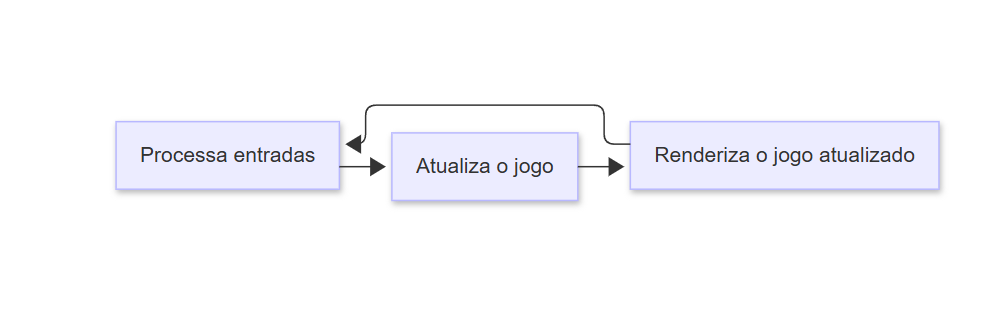
\includegraphics[scale=0.7]{imagens/LoopEngineJogo.png}
	\\\textbf{Fonte:} Adaptado de \cite{Alves2020}
	\label{fig:ciclovidajogo}
\end{figure}
\FloatBarrier


\subsection{\textit{Godot Engine}}

A \textit{Godot Engine} é uma ferramenta grátis e de código aberto licenciado pelo MIT para criação de jogos 2D e 3D \cite{godot_docs},
a \textit{Godot Engine} oferece ao desenvolvedor ferramentas para criação de jogos, gereciamento de \textit{assets} e também oferece um editor de script integrado,
o desenvolvimento na \textit{Godot Engine} é baseado em classes de objetos chamados nós (\text{nodes}) \cite{salmela2022_godot, godot_docs}. 
Existem muitos tipo de nós disponíveis, nós para gráficos, física, interface de usuário, audio e de outros tipos, esses 
nós são organizados em uma cena conforme o desenvolvedor quiser para comportamentos mais complexos \cite{salmela2022_godot, godot_docs},
assim como um script pode ser anexado a um nó para também conseguir um comportamento específico. \textit{Godot Engine} tem uma linguagem para programar
scripts chamada GDScript, a síntaxe é bem similar ao Python por causa da indentação mas não é baseado na mesma, também uporta a linguagem C\# \cite{godot_docs}.
Um exemplo do ambiente de desenvolvimento na \textit{Godot Engine} é mostrado na figura~\ref{fig:janelaGodot} abaixo:

\FloatBarrier
\begin{figure}[!htbp]
	\centering
	\caption{Janela do editor Godot durante o desenvolvimento do jogo}
	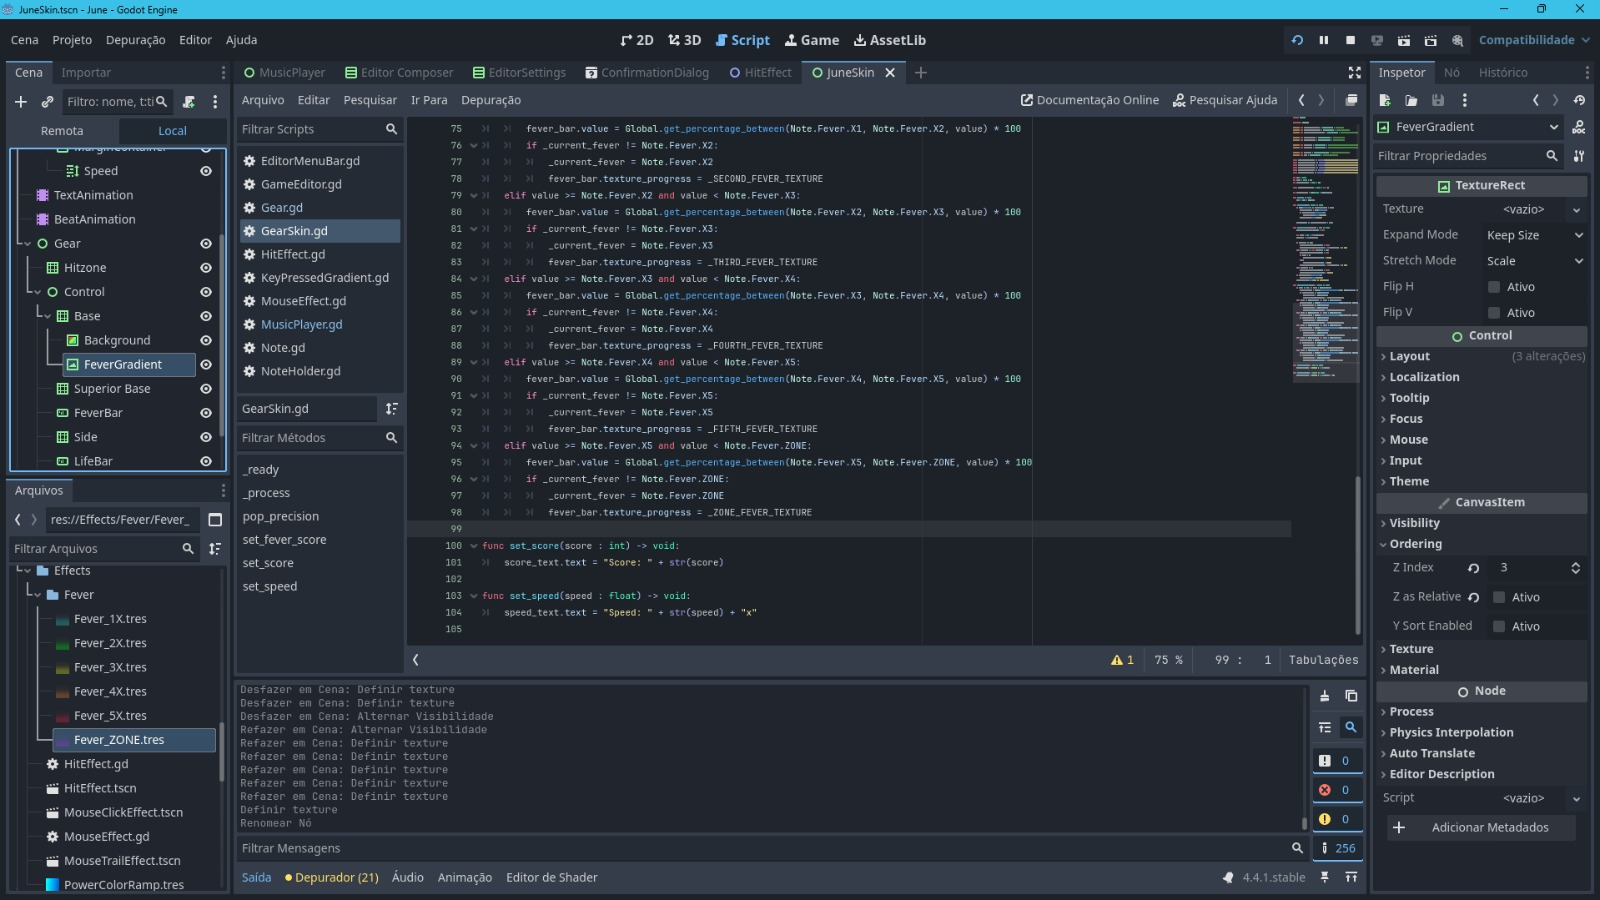
\includegraphics[scale=0.3]{imagens/Godot.jpg}
	\\\textbf{Fonte:} Elaborado pelo Autor
	\label{fig:janelaGodot}
\end{figure}
\FloatBarrier

\textit{Godot Engine} possui fluxos separados de renderização 2D e 3D, 
na renderização 3D oferece físicas de sombra e luz, 
já na renderização em 2D também oferece luz, sombra e máscaras. 
Em ambos os fluxos de renderização possibilita o desenvolvedor utilizar físicas para simulação e 
\textit{ray casting}\footnote{Técnica de renderização 3D a partir de um ponto de observação} \cite{godot_docs}.



\subsection{Java}

Java é uma linguagem de programação de baixo nível que surgiu na década de 90, como uma necessidade para tráfegar dados na web, a linguagem é baseada no paradigma de orienteção à objeto, 
é possível encapsular dados dentro de um bloco e criar métodos de manipulação desses dados. Um exemplo de encapsulamento é mostrado na figura~\ref{fig:encapsulamento} abaixo: 

\FloatBarrier
\begin{figure}[!htbp]
	\centering
	\caption{Encapsulamento de variáveis e métodos}
	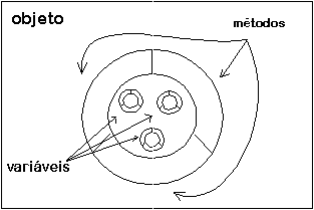
\includegraphics[scale=1]{imagens/EncapsulamentoObjetoJava.png}
	\\\textbf{Fonte:} \cite{indrusiak_java}
	\label{fig:encapsulamento}
\end{figure}
\FloatBarrier

Um exemplo em código de encapsulamento:

\lstinputlisting[language=Java]{fontes/Classe.java} 

A linguagem também permite a modularização das aplicações, reuso e manuntenção simples do código implementado \cite{indrusiak_java}.
Sob as camadas internas, Java em seus recursos fundamentais de uma linguagem, como estruturas de controles, estruturas de definição,
tratamentos de exceções, construtores de objeto, modificadores de acesso, tipos de dados e outros, é padronizado e mantém um 
conjunto de recursos limitado comparado á outras linguagens, essa padronização e simplicidade se mostra na ausência no uso 
de ponteiros e gerenciamento de memória por meio da programação, fazendo com que a programação fique mais eficiente \cite{indrusiak_java}. 

A linguagem Java é tanto interpretada como compilada, após escrever um código em Java, é salvo o arquivo fonte e em seguida é possível
compilar este arquivo fonte, produzindo um arquivo binário chamado de arquivo classe, esses arquivos não são executados diretamente pelos processadores,
esses arquivos estão em um formato chamado \textit{bytecode} e assim podem ser executados em qualquer interpretador de Java, o código precisa ser compilado 
apenas uma vez, pois os \textit{bytecode} são gerados dentro do arquivo classe e podem ser executados em qualquer plataforma de hardware e software \cite{indrusiak_java, deitel2016java}, é mostrado mais detalhadamente na figura~\ref{fig:javacompilador} abaixo:

\FloatBarrier
\begin{figure}[!htbp]
	\centering
	\caption{Como funciona a execução e compilação de um código em java}
	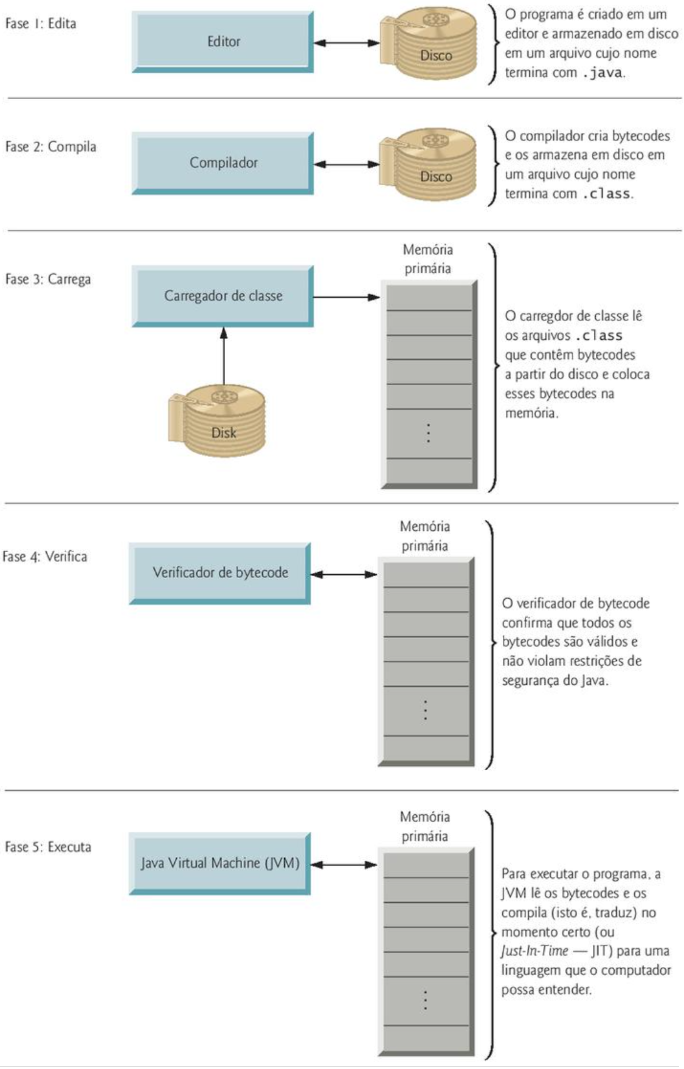
\includegraphics[scale=0.6]{imagens/CompiladorJava.png}
	\\\textbf{Fonte:} \cite{deitel2016java}
	\label{fig:javacompilador}
\end{figure}
\FloatBarrier

\subsubsection{LibGDX}

LibGDX é um framework\footnote{Conjunto de ferramentas, bibliotecas, componentes prontos e boas práticas que fornecem uma estrutura base para o desenvolvimento de software.} 
escrito em java, utiliza OpenGL \footnote{Interface de programação de aplicações (API) gráfica multiplataforma que permite renderizar gráficos 2D e 3D. Disponível em:https://www.opengl.org/} e 
é código aberto para desenvolvimento de jogos 3D e 2D para computadores e celulares \cite{libgdx_wiki},
a LibGDX oferece módulos para que a arquitetura de um jogo possa ser construído, são eles:
\begin{itemize}
	\item \textbf{Módulo de entradas:} Dá ao desenvolvedor uma forma unificada 
	de modelos de entradas, detectando teclados, telas sensíveis ao toque, aceletometros e mouses \cite{libgdx_wiki}.
	\item \textbf{Módulo de gráficos:} Proporciona o desenho de imagens na tela utilizando OpenGL ES\footnote{(Graphics Library for Embedded Systems) Disponível em: https://www.khronos.org/opengles/} fornecido por hardware \cite{libgdx_wiki}.  
	\item \textbf{Módulo de arquivos:} Concede o acesso a métodos convenientes para leitura e gravação de arquivos de mídia \cite{libgdx_wiki}.
	\item \textbf{Módulo de áudio:} Disponibiliza recursos de áudio para gravação e reprodução de arquivos áudio em todas as plataformas \cite{libgdx_wiki}.
	\item \textbf{Módulo de redes:} Fornece ao desenvolvedor metódos para utilizar recursos de rede, 
	usando protocolos de internet e comunicação cliente e servidor \cite{libgdx_wiki}.
\end{itemize}

Com esses módulos disponíveis na biblioteca LibGDX, abaixo na figura~\ref{fig:ciclolibgdx} mostra um diagrama como esses módulos são usados em um ciclo de vida de um jogo:

\FloatBarrier
\begin{figure}[!htbp]
	\centering
	\caption{Ciclo de vida de um jogo com os módulos da LibGDX}
	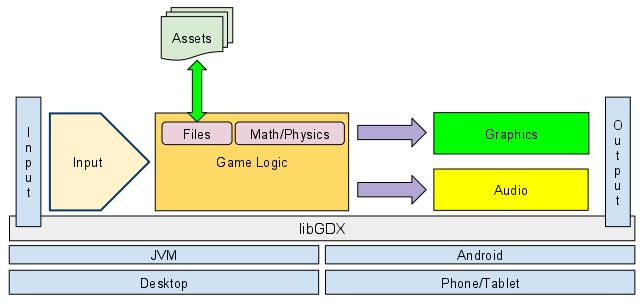
\includegraphics[scale=0.8]{imagens/CicloDeVidaJogo.png}
	\\\textbf{Fonte:} \cite{libgdx_wiki}
	\label{fig:ciclolibgdx}
\end{figure}
\FloatBarrier

Além disso, LibGDX oferece ao desenvolvedor a possibilidade de utilizar partículas 2D,
manipulação de \textit{bitmaps} e editor de texturas, junto com isso \cite{libgdx_wiki, firmansyahRPGLibgdx}, existem métodos principais, são essenciais para manter o ciclo de vida de um jogo, são eles na tabela~\ref{metodos} abaixo:

\FloatBarrier
\begin{table}[!htbp]
	\centering
	\caption{Ciclo de Métodos do LibGDX }
	\begin{tabular}{ c | p{10cm} }
		\hline
		\textbf{Nome do Método} & \textbf{Descrição} \\ \hline
		\textbf{Create()} & Este método será usado uma vez quando a aplicação for criada.           \\ \hline
		\textbf{Resize(int width, int height)} & Este método será sempre usado quando o tamanho da tela do jogo estiver mudando e não estiver em pausa. Há um parâmetro de largura e altura da tela que é atualizado sempre que o jogo for redimensionado.          \\ \hline
		\textbf{Render()} & Este método é usado como repetição do jogo na aplicação. A lógica do jogo é atualizada aqui.           \\ \hline
		\textbf{Pause()} & No Android, este método é usado quando o botão \textit{home} é pressionado ou quando há uma chamada telefônica. No desktop, este método é usado apenas uma vez antes do método \textit{dispose}.           \\ \hline
		\textbf{Resume()} & Este método é usado apenas no Android para continuar a aplicação após estar em pausa.          \\ \hline
		\textbf{Dispose()} & Este método é usado para fechar a aplicação.           \\ \hline
	\end{tabular}
	\\ \vspace{0.2cm}
	\textbf{Fonte:} Adaptado de \cite{firmansyahRPGLibgdx}
	\label{metodos}
\end{table}
\FloatBarrier

\subsection{C++}

A linguagem de programação C++ de alto nível, se originou a partir da linguagem de programação C, foi criado para abstrair dados, suportar a programação orientada a objeto e suprir uma 
demanda de programas de softwares que ocorreu na década de 1980 \cite{deitel2005cpp, overviewCPP}.

C++ é uma linguagem que mistura tanto a programação orientada a objeto tanto quanto a programação procedural, assim o programador tem uma
maior flexibilidade escolhendo o paradigma que mais se adequa ao projeto, a criação de códigos fica mais eficiente e é mais reutilizáveis por causa da 
modularização\footnote{Tarefas separadas em funções ou procedimentos, cada uma realizando uma parte do programa}.

Os programas em C++ são feitos classes e funções existentes na C++ \textit{Standart Library}, além disso a linguagem suporta a programação genérica
por meio de modelos de diferentes tipos, sem a necessidade de reescrever o código\cite{turos2024cpp, deitel2005cpp}.

Os códigos feitos em C++ ao serem executados passam por 6 fases: edição, pré-processamento, compilação, linkagem, carregamento e execução, como mostrado na figura~\ref{fig:compiladorCplus} abaixo:

\FloatBarrier
\begin{figure}[!htbp]
	\centering
	\caption{As fases para rodar um código em C++}
	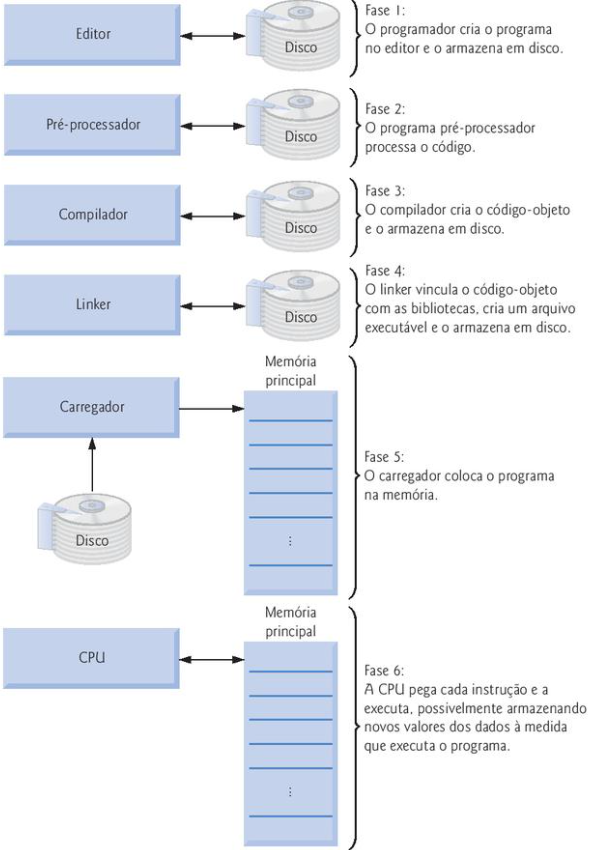
\includegraphics[scale=0.8]{imagens/ambienteC.png}
	\\\textbf{Fonte:} \cite{deitel2005cpp}
	\label{fig:compiladorCplus}
\end{figure}
\FloatBarrier



\subsubsection{Raylib}

Raylib é uma biblioteca de programação de Jogos 2D e 3D de código aberto escrita em C.
A Raylib não provê uma API de documentação igual o Godot ou a LibGDX, apenas uma lista com todas funções disponíveis e um exemplo de como usa-las, Raylib tem suporte para computadores, tanto Desktop quanto para Web e para celulares,
apesar de ser escrita em C, a linguagem suporta também pode ser usada em linguagens como C++ e Python \cite{raylib2025}.
Assim como a LibGDX e o godot, a Raylib tem funções próprias que compõe a arquitetura de um jogo \cite{raylib2025}, abaixo na tabela~\ref{funcoesraylib} é mostrado as funções e o que fazem:

\FloatBarrier
\begin{table}[!htbp]
	\centering
	\caption{Funções básicas para utilizar a raylib}
	\begin{tabular}{ c | p{6cm} }
		\hline
			\textbf{Nome da função} & \textbf{Descrição} \\ \hline
			\textbf{ InitWindow(Width, Height, "My Game")} & Este método será usado uma vez quando a aplicação for criada. Há parâmetro de largura e altura da tela e o nome da janela  \\ \hline
			\textbf{ SetTargetFPS(60)} & Este método configura quantos quadros por segundo o jogo será renderizado \\ \hline
			\textbf{ BeginDrawing()} & Este método é usado dentro de uma estrutura de \textit{loop}, serve para desenhar na janela \\ \hline
			\textbf{ ClearBackground(RAYWHITE)} & Este método é usado para limpar a janela em uma cor específica para evitar erros visuais \\ \hline
			\textbf{ EndDrawing()} & Este método é utilizado para terminar o desenho dentro da janela \\ \hline
			\textbf{ CloseWindow()} & Método para fechar a aplicação \\ \hline
	\end{tabular}
	\\ \vspace{0.2cm}
	\textbf{Fonte:} Elaborada pelo autor com base em \cite{raylib2025}
	\label{funcoesraylib}
\end{table}
\FloatBarrier

Também abaixo é mostrado um código base para a programação de um jogo em Raylib:

\lstinputlisting[language=C++]{fontes/Raylib.cpp} 

\subsection{Python}

Python é uma linguagem de alto nível que surgiu na década de 1990 especializada para físicos e engenheiros, é usada popularmente nos dias atuais por empresas alta tecnologia, 
diferentemente de várias outras linguagens de programação populares, python o código precisa ser bem indentado pois depende do recuo para 
o código funcionar, o que torna a linguagem com sintaxe simples, clara e concisa\cite{thinkPython, oracle2025_python}, na figura~\ref{fig:indentacaopython} abaixo é demonstrado essa indentação:

\FloatBarrier
\begin{figure}[!htbp]
	\centering
	\caption{Indentação de um programa comum em python}
	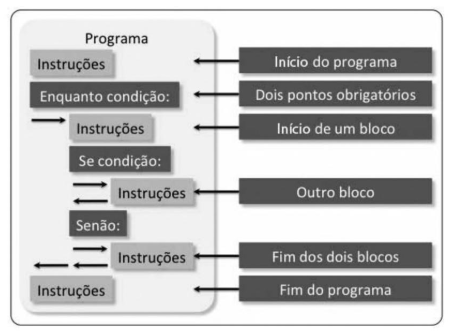
\includegraphics[scale=0.8]{imagens/EstruturaProgramaPython.png}
	\\\textbf{Fonte:} \cite{pythonDesenvolvedores}
	\label{fig:indentacaopython}
\end{figure}
\FloatBarrier

Python é interpretada, ou seja, não é criado um arquivo com uma linguagem de máquina para o computador ler, 
o código é lido por um interpretador na máquina virtual python \cite{thinkPython}, como mostrado na figura~\ref{fig:interpretadorpython} abaixo:

\FloatBarrier
\begin{figure}[!htbp]
	\centering
	\caption{Diagrama de um interpretador}
	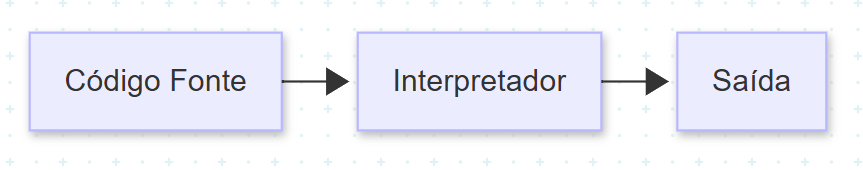
\includegraphics[scale=0.5]{imagens/Interpretador.png}
	\\\textbf{Fonte:} adaptado de \cite{thinkPython}
	\label{fig:interpretadorpython}
\end{figure}
\FloatBarrier

A linguagem possui diversas estruturas e uma grande coleção de módulos prontos para uso, como listas, dicionários, data/hora, e outros recursos, inclusive é possivel adicionar frameworks e bibliotecas de terceitos \cite{pythonDesenvolvedores},
além disso, python é considerado uma linguagem de multi-paradigmas, ela suporta a programação modular, procedural, funcional e a orientada à objetos \cite{ParadigmsPython}. Abaixo está um exemplo de um programa simples em python:

\lstinputlisting[language=python]{fontes/programa.py} 

\subsubsection{Pygame}

Pygame é um framework para Python, foi feita sobre a biblioteca SDL(Simple DirectMedia)\footnote{Biblioteca de desenvolvimento em C para recursos de áudio, teclado, mouse e gráficos. Disponível: https://www.libsdl.org/}
que permitiu abstrair os recursos da biblioteca para que fosse mais acessível e mais fácil o desenvolvimento de jogos, através de módulos é possivel construir uma estrutura para um jogo \cite{pygame2025},
todos os métodos da biblioteca são chamados pela biblioteca pygame, abaixo tem a tabela~\ref{pygame} exemplificando:
\cite{pygame2025}

\FloatBarrier
\begin{table}[!htbp]
	\centering
	\caption{Funções principais da biblioteca Pygame.}
	\begin{tabular}{ c | p{6cm} }
		\hline
			\textbf{Função} & \textbf{Descrição} \\ \hline
			\textbf{pygame.init()} & Importa e inicializa todos os módulos da biblioteca. \\ \hline
			\textbf{pygame.display} & Vários métodos para configurar a janela ou a tela \\ \hline
			\textbf{pygame.event.get()} & Detecta se algum evento ocorreu, por exemplo: jogador apertou uma tecla. \\ \hline
			\textbf{pygame.draw} & Conjunto de métodos usados para desenhar formas e geometria. \\ \hline
			\textbf{pygame.display.flip()} & Atualiza a tela inteira. \\ \hline
			\textbf{pygame.quit()} & Fecha a aplicação. \\ \hline
	\end{tabular}
	\\ \vspace{0.2cm}
	\textbf{Fonte:} Elaborada pelo autor com base em \cite{pygame2025}
	\label{pygame}
\end{table}
\FloatBarrier

\section{Trabalhos Correlatos}
\subsection{Desenvolvimento de jogos eletrônicos}

No trabalho de \cite{morais2009jogos} propõe um estudo de um desenvolvimento de um jogo chamado "\textit{I Wanna be the
Tribute}" feito com o motor gráficos do Game Maker 7.0, o autor aborda técnicas e o processo de engenharia de Software 
no desenvolvimento de um jogo.

No trabalho de \cite{morais2009jogos} afirma que o processo de desenvolvimento de jogos eltrônicos possui 5 fases, elas são:

\begin{itemize}
	\item \textbf{\textit{Game Design:}} O \textit{game design} é a etapa mais importante na hora de construir um 
	jogo, com ela, é definido a forma como o jogador pensa e raciocina para tomar decisões que cheguem à um objetivo 
	e essas decisões são tomadas a partir da regra do jogo. Segundo as palavras de \cite{morais2009jogos}:
		\begin{citacao}
			Um design mal feito vai gerar um jogo ruim, sem dúvidas, e este problema deve-se ao fato de que o game design ainda é uma idéia muito nova na indústria. Um game design inovador geralmente traz um bom retorno
		\end{citacao}
	\item \textbf{Conceitualização:} Antes de começar o desenvolvimento do jogo, 
	o criador deve pensar como o jogo deve ser, quais os objetivos do jogador e que desafios ele irá encontrar para alcança-los.
	Ao longo do desenvolvimento pode haver mudança que não está na conceitualização.
	\item \textbf{Imersão:} Um jogo propõe ao jogador um novo mundo fictício com regras próprias para se imergir nele, 
	tanto o mundo quanto as regras devem fazer sentido para que seja imersivo. Um mundo estático com personagens mal planejados e sem personalidade,
	 com uma história mal elaborada, geralmente termina em um jogo ruim.
	\item \textbf{Desenho:} A aparência visual de um jogo, que inclui o design dos cenários e dos personagens, é importante porque é o que 
	permite ao jogador ver e interagir com o mundo virtual. Por isso, é essencial que a parte gráfica seja bem elaborada e bem feita.
	\item \textbf{Inteligência Artificial:} Nas maiorias dos jogos não há apenas o jogador naquele universo, há os não-jogadores, 
	que são as inteligências artificiais, existem várias formas de se utilizar IA em jogos, mas o mais utilizado é o modelo básico, máquinas de estados finitos,
	de acordo com o ambiente e o jogador é feita uma decisão/ação.
	\item \textbf{Programação:} A programação é feita a partir de uma linguagem e em conjunto a linguagem é usada uma API (\textit{Application
	Programming Interface}) como DirectX e OpenGL, para dar suporte à linguagem, com funções e módulos de cálculo de colisão, física de um
ambiente, configuração de sons e vídeo que ajudam no desenvolvimento.
\end{itemize}

A proposta no desenvolvimento do jogo de \cite{morais2009jogos} é que o jogo é 2D e propõe o \textit{game design} que o jogador aprende ao perder,
com a experiencia da derrota anterior, o jogador obtem conhecimento do ambiente e das regras para conseguir chegar no objetivo.

A conclusão para o trabalho de \cite{morais2009jogos} é que um projeto de desenvolver um jogo se difere em vários aspectos da engenharia de software, por 
necessitar da criatividade para um bom \textit{game design}, segundo \cite{morais2009jogos}:
\begin{citacao}
	Um bom game design não só gera um bom jogo, mas também 
	um bom game designer, que são aqueles que se 
	dedicam ao estudo das técnicas propostas neste 
	trabalho, desde a concepção das idéias até o 
	desenho do ambiente, da interface homem máquina, e do balanceamento do jogo.
\end{citacao}

\subsection{Estudo comparativo entre engines de desenvolvimento de jogos 2D}

O trabalho de \cite{Alves2020} visou comparar dois motores gráficos para o desenvolvimento de jogos 2D para celulares, Unity e a Construct 3,
o jogo em si focou em ser simples e abrangente para que as caracteristicas técnicas dos motores gráficos e fossem coletadas e analisádas, tendo como objetivos específicos:
\begin{itemize}
	\item Estudar as características técnicas das 2 \textit{engines} para desenvolver o jogo;
	\item Desenvolver 2 jogos nas duas \textit{engines};
	\item Avaliar os dados analisados e coletados dos 2 jogos feitos nas 2 \textit{engines};
\end{itemize}

Foi feito um \textit{Game Desing Document} para o maior entendimento do que seria o jogo 
à ser desenvolvido, levantando os aspectos mais importantes pro desenvolvedor.
As métricas à serem avaliadas afim de comparar o desenvolvimento nas \textit{engines} foram: 

\begin{enumerate}
	\item \textit{TilesMap}: \textit{Tiles} são cada bloco repetitivos que constituirão o piso e paredes de cada nível do jogo;
	\item Sistema de câmera: Visão apresentado para o jogador no momento atual aonde está o personagem;
	\item Movimentação do jogador: O movimento do jogador é a mudança de posição do avatar do jogador no \textit{Tiles} recentemente criados;
	\item Sistema de luz: Sistema de luz simula a luz real, em que uma fonte luz clareia uma determinada área;
	\item Sistema de movimentação de IA: O movimento dos inimigos até o jogador de maneira automática;
	\item Sistema de som: Processo da aplicação de tocar algum som quando determinada ação acontece;
	\item Transição de Fases: Transição de uma fase do jogo para outra.
\end{enumerate}

A escolhas dessas métricas segundo \cite{Alves2020} está diretamente relacionado ao ascpectos de desenvolvimento.

Foi desenvolvido em ambos motores gráficos um jogo chamado "A luz no fim do túnel", de gênero \textit{puzzle}, 2D e \textit{top-down}
em que o jogador se encontrar em um labirinto com inimigos e armadilhas.

O estudo de \cite{Alves2020} concluiu que o desenvolvimento na Construct 3 
foi mais simples devidos algumas ferramentes presentes na \textit{engine} e foi se utilizado scripts em JavaScript, 
já a Unity se mostrou mais complexa e mais completa que a Construct 3, pórem devido a comunidade envolta da Unity é maior,
portanto houve  mais alternativas de conteúdo para resolução de problemas durante a fase de desenvolvimento.
Foi se observado também que para construção do executável do jogo, a disponibilização na Unity é gratuita, mas na Construct 3 o desenvolvedor
é obrigado a pagar a licença anual.

\subsection{Estudo comparativo de motores de jogos no desenvolvimento de um jogo 2D para web}

O trabalho se inicia com \cite{pantoja2022jogos} explicando a relevância dos jogos para web e que a partir deste cenário, 
o trabalho terá como objetivo desenvolver um jogo 2D avaliando os motores de jogos utilizados durantes desenvolvimento, sendo assim, um estudo comparativo.

Foi feito uma pesquisa no \textit{Google Trends} para escolher e filtrar os motores de jogos mais utilizados, quais exportam os jogos para web e 
quais atendem ao requisito mínimo que seria um notebook k Dell
Inspiron 5537 Intel(R) Core(TM) i7-4500U CPU @ 1.80GHZ (4 CPUs) 2.40GHZ, 8GB Memória
RAM, também foi feito um \textit{Game Design Document} para levantar os requisitos e aspectos primordiais do jogo a ser desenvolvido.

Como resultado os apenas as \textit{Unity} e \textit{Godot} foram selecionados para o desenvolvimento do jogo.
O jogo desenvolvido se chama "Os mortos-vivos" do genêro ação, no qual o jogador derrota hordas de inimigos, coleta experiência e sobe de nível.

Foram utilizados algumas métricas para realizar a avaliação dos motores, métricas para o código fonte e métricas para performance:
Para o código fonte:
\begin{enumerate}
	\item Tamanho final do arquivo;
	\item Quantidade de arquivos de código;
	\item Quantidade de linhas;
	\item Quantidade de linhas de código;
	\item Complexidade do código.
\end{enumerate} 
Para a perfomance:
\begin{enumerate}
	\item Tempo de carregamento de jogo;
	\item Uso de CPU mínimo;
	\item Uso de CPU máximo;
	\item Média do uso de CPU;
	\item Uso de memória RAM mínimo;
	\item Uso de memória RAM máximo;
	\item Média do uso de memória RAM.
\end{enumerate} 

O estudo comparativo de \cite{pantoja2022jogos} foi concluído que entre os motores \textit{Unity} 
e \textit{Godot} evidencia diferenças significativas em termos de usabilidade e desempenho. 
O \textit{Godot} apresenta menor complexidade, exigindo menos linhas de código e sendo mais 
acessível para iniciantes no desenvolvimento de jogos. Já a \textit{Unity}, embora mais 
complexo, demonstrou desempenho superior durante os testes, com maior 
estabilidade em cenários variados. Assim, o \textit{Godot} é recomendado para iniciantes, 
enquanto a \textit{Unity} se mostra mais adequado para projetos que priorizam funcionalidades 
complexas e uma melhor experiência do jogador.
